\documentclass{crceitthesis-3}
\usepackage{longtable} %for long tables to be fitted on multiple pages
\usepackage{ragged2e}
%\usepackage{color}
\usepackage{graphicx}
\usepackage{varioref}
\usepackage{epsfig}
\usepackage{times}
\usepackage[section]{placeins} % to keep floats(figures) in the section in which they were issued
\usepackage{amsmath}
\usepackage{amssymb}
\usepackage{url}
\usepackage{multirow}
\usepackage[T1]{fontenc}
\usepackage{ascii}
\usepackage{nomencl}
\usepackage{lscape}
\usepackage{longtable,tabu}
\usepackage{lmodern}
\usepackage{lipsum}
\usepackage[tight,footnotesize]{subfigure}
\usepackage{cite}
\usepackage[acronym]{glossaries} 
\usepackage{fancybox}
\usepackage{algorithmic}
\usepackage[boxed]{algorithm}
\usepackage[compact]{titlesec}
\usepackage{gensymb}
\usepackage{multicol}
%----------For code listing---------------------------------------------------
\usepackage{listings} % Required for inserting code snippets
\usepackage[usenames,dvipsnames]{color} % Required for specifying custom colors and referring to colors by name

\definecolor{DarkGreen}{rgb}{0.0,0.4,0.0} % Comment color
\definecolor{highlight}{RGB}{255,251,204} % Code highlight color

\lstdefinestyle{Style1}{ % Define a style for your code snippet, multiple definitions can be made if, for example, you wish to insert multiple code snippets using different programming languages into one document
language=Scilab, % Detects keywords, comments, strings, functions, etc for the language specified
backgroundcolor=\color{highlight}, % Set the background color for the snippet - useful for highlighting
basicstyle=\footnotesize\ttfamily, % The default font size and style of the code
breakatwhitespace=false, % If true, only allows line breaks at white space
breaklines=true, % Automatic line breaking (prevents code from protruding outside the box)
captionpos=b, % Sets the caption position: b for bottom; t for top
commentstyle=\usefont{T1}{pcr}{m}{sl}\color{DarkGreen}, % Style of comments within the code - dark green courier font
deletekeywords={}, % If you want to delete any keywords from the current language separate them by commas
%escapeinside={\%}, % This allows you to escape to LaTeX using the character in the bracket
firstnumber=1, % Line numbers begin at line 1
frame=single, % Frame around the code box, value can be: none, leftline, topline, bottomline, lines, single, shadowbox
frameround=tttt, % Rounds the corners of the frame for the top left, top right, bottom left and bottom right positions
keywordstyle=\color{Blue}\bf, % Functions are bold and blue
morekeywords={}, % Add any functions no included by default here separated by commas
numbers=left, % Location of line numbers, can take the values of: none, left, right
numbersep=10pt, % Distance of line numbers from the code box
numberstyle=\tiny\color{Gray}, % Style used for line numbers
rulecolor=\color{black}, % Frame border color
showstringspaces=false, % Don't put marks in string spaces
showtabs=false, % Display tabs in the code as lines
stepnumber=5, % The step distance between line numbers, i.e. how often will lines be numbered
stringstyle=\color{Purple}, % Strings are purple
tabsize=2, % Number of spaces per tab in the code
}

% Create a command to cleanly insert a snippet with the style above anywhere in the document
\newcommand{\insertcode}[2]{\begin{itemize}\item[]\lstinputlisting[caption=#2,label=#1,style=Style1]{#1}\end{itemize}} % The first argument is the script location/filename and the second is a caption for the listing

%--------------------------------------End of code listing-------------------

\titlespacing{\section}{0pt}{2ex}{1ex}
\titlespacing{\subsection}{0pt}{1ex}{0ex}
\titlespacing{\subsubsection}{0pt}{0.5ex}{0ex}

\usepackage[compact]{titlesec}
\titleformat{\chapter}[display]
  {\normalfont\huge\bfseries\centering}{\chaptertitlename\ \thechapter}{20pt}{\LARGE}

%\usepackage[toc,page]{appendix}

\makeglossaries
\makenomenclature

\newglossaryentry{wsn}{name=WSN,description=Wireless Sensor Network}
\newglossaryentry{manet}{name=MANET,description=Mobile Ad hoc NETwork}
\newglossaryentry{gps}{name=GPS,description=Global Positioning System}
\newglossaryentry{spin}{name=SPIN,description=Sensor Protocols for Information via Negotiation}
\newglossaryentry{dc}{name=DC,description=Data Centric}
\newglossaryentry{bs}{name=BS,description=Base Station}
\newglossaryentry{mcfa}{name=MFCA,description=Minimum Cost Forwarding Algorithm}
\newglossaryentry{acquire}{name=ACQUIRE,description=Active Qwery Forwarding in Sensor Networks}
\newglossaryentry{leach}{name=LEACH,description=Low Energy Adaptive Clustering Hierarchical}
\newglossaryentry{leachc}{name=LEACH-C,description=LEACH Centralized}
\newglossaryentry{pegasis}{name=PEGASIS,description=Power Efficient Gathering in Sensor Information Systems}
\newglossaryentry{teen}{name=TEEN,description=Threshold-Sensitive Energy Efficient SensormNetwork Protocol}
\newglossaryentry{heed}{name=HEED,description=Hybrid Energy-Efficient Distributed}
\newglossaryentry{gaf}{name=GAF,description=Geographic Adaptive Fidelity}
\newglossaryentry{gear}{name=GEAR,description=Geographic and Energy Aware Routing}
\newglossaryentry{sleachc}{name=sLEACH-C,description=Solar-aware LEACH-centralized extension}
\newglossaryentry{group}{name=GROUP,description=Genetic algorithm inspired ROUting Protocol}
\newglossaryentry{aco}{name=ACO,description=Genetic algorithm inspired ROUting Protocol}
\newglossaryentry{pso}{name=PSO,description=Particle swarm optimization}

\newglossaryentry{aodv}{name=AODV,description=Ad hoc On-demand Distance Vector}
\newglossaryentry{dsr}{name=DSR,description=Dynamic Source Routing}
\newglossaryentry{rfc}{name=RFC,description=Request For Comments}
\newglossaryentry{ara}{name=ARA,description=Ant-Inspired Routing Algorithm}
\newglossaryentry{ec}{name=EC,description=Evolutionary Computation}
\newglossaryentry{ga}{name=GA,description=Genetic Algorithms}
\newglossaryentry{ils}{name=ILS,description=Iterated Local Search}
\newglossaryentry{sa}{name=SA,description=Simulated Annealing}
\newglossaryentry{ts}{name=TS,description=Tabu Search}
\newglossaryentry{si}{name=SI,description=Swarm Intelligence}
\newglossaryentry{as}{name=AS,description=Ant System}
\newglossaryentry{eas}{name=EAS,description=Elitist strategy for Ant System}
\newglossaryentry{tsp}{name=TSP,description=Traveling Salesman Problem}
\newglossaryentry{so}{name=SO,description=Self-Organization}
%%%%%%%%%%%%%%%%%%%%%%%%%%%%%MAIN PART OF THE REPORT%%%%%%%%%%%%%%%%%%%%%%%%%%%%%%%
\begin {document}
\graphicspath{{./}{images/}}
\headheight-8pt % to adjust white space.
\headsep -12pt %
\footskip 18mm %
% prelude.tex
%   - titlepage
%   - dedication (optional)
%   - approval sheet
%   - table of contents, list of tables and list of figures
%   - abstract
%============================================================================


\clearpage\pagenumbering{roman}  % This makes the page numbers Roman (i, ii, etc)


% TITLE PAGE
%   - define \title{} \author{} \date{}
\title{Smart Energy Monitor}
\stua{Shabbir Ahmed}
\stub{Dylan Dcruz}
\stuc{Jonathan Pereira}

\date{\large March 17, 2018} %\today

%  - Roll number, required for title page, approval sheet, and
%    certificate of course work 

\rollnuma{7173}
\rollnumb{7304}
\rollnumc{7337}

%   - The default degree is ``Doctor of Philosophy''
%     (unless the document style msthesis is specified
%      and then the default degree is ``Batchlor of Engineering'')
%     Degree can be changed using the command \mudegree{}
\mudegree{Bachelor of Engineering}


%   - The default report type is preliminary report.
%      * for a PhD thesis, specify \thesis
%\thesis
%      * for a M.Tech./M.Phil./M.Des./M.S. dissertation, specify \dissertation
\project
%      * for a DIIT/B.Tech./M.Sc.project report, specify \project
%\project
%      * for any other type, use  \reporttype{}
%\reporttype{ReportType}

%   - The default department is ``Unknown Department''
%     The department can be changed using the command \department{}
\department{DEPARTMENT OF ELECTRONICS}

%\section{Graphics}
%    - Set the guide's name
\setguide{Prof. Jayen Modi}
%    - Set the coguide's name (if you have one)
%\setcoguide{PPP}
%    - Set external guide (if you have one)
%\setexguide{Prof External Guide}

%   - once the above are defined, use \maketitle to generate the titlepage
\maketitle

%--------------------------------------------------------------------%
% DEDICATION
%   Dedications, if any, must be first page after title page.
\begin{dedication}
 \bf \it 
%I appreciate and am very thankful for their continued motivation and support. 
\end{dedication}

%--------------------------------------------------------------------%
% APPROVAL SHEET
%   - for final thesis, you need Approval Sheet. So, uncomment the
%     \makeapproval command.
%     it should come after dedication, if dedication is
%     present. Otherwise it is the first page after title page.

\makecertificate

\makeapproval



%--------------------------------------------------------------------%
% COPYRIGHT PAGE
%   - To include a copyright page use \copyrightpage
% \copyrightpage

%--------------------------------------------------------------------%
% ABSTRACT

\thispagestyle{empty}
%\input{declaration.tex}
\makedeclaration
\begin{titlepage}
\thispagestyle{empty}
%\pagestyle{empty}
\begin{center}
\begin{LARGE}
\bf {Abstract}
\end{LARGE}

\end{center}
\large
In 2014, the Electricity Consumption per capita in India was 805.6KWh which is equivalent to 637.43 kg of oil per capita. Over 58 percent of this electricity is produced from non renewable sources of energy. Our dependence on production of energy from non renewable sources of energy makes India both a major greenhouse gas emitter and one of the most vulnerable countries in the world to projected climate change. The country is already experiencing changes in climate and the impacts of climate change, including water stress, heat waves and drought, severe storms and flooding, and associated negative consequences on health and livelihoods. It is imperative that India rapidly adopts renewable sources of energy like solar and wind. But in addition to that it is also the responsibility of the Indian people to monitor their energy consumption and reduce their carbon footprint. 
The Smart Energy Monitor helps the Indian consumer to reduce and monitor their household energy consumption by providing insights to consumption of electricity by individual electrical appliances. The Smart Energy Monitor  connects directly to your electricity panel and uses a mobile app to tell you what devices and appliances are drawing power and when. The monitor listens to the electronic signature of each device and uses algorithms to identify them and monitor their power consumption. It also presents real-time and historical usage for each device. It will help the consumer track energy inefficient appliances and also their monthly usage. From these insights the consumer can reduce their electricity consumption thereby reducing their carbon footprint. 





\end{titlepage}


%--------------------------------------------------------------------%
% CONTENTS, TABLES, FIGURES
%\tableofcontents
%\listoftables
%\listoffigures

%--------------------------------------------------------------------%
% NOMENCLATURE
%\begin{nomenclature}
%\begin{description}
%\item{\makebox[0.75in][l]{$C_1$}} Constant 1
%
%\item{\makebox[0.75in][l]{$V$}}    Voltage 
%
%\item{\makebox[0.75in][l]{\$}}     US Dollars
%\end{description}
%\end{nomenclature}
%
%\cleardoublepage\pagenumbering{arabic} % Make the page numbers Arabic (1, 2, etc)
   %%Make changes in this file for title of the project, abstract and details of the author
\begin{acknowledgments}

\thispagestyle{empty}

\noindent We have great pleasure in presenting the report on {\bf "\projecttitle"}. I take this opportunity to express my sincere thanks towards the guide Prof. Jayen Modi, C.R.C.E, Bandra (W), Mumbai, for providing the technical guidelines, and the suggestions regarding the line of this work. We enjoyed discussing the work progress with him during our visits to department.\\

\noindent We thank Dr. Deepak V. Bhoir, Head of Electronics Dept., Principal and the management of C.R.C.E., Mumbai for encouragement and providing necessary infrastructure for pursuing the project.\\

\noindent We also thank all non-teaching staff for their valuable support, to complete our project.
\par
%

%\hfill 

\end{acknowledgments}
%I thank the many people who have done lots of nice things for me.



\newpage
\tableofcontents
\listoffigures
%\listoftables
\printglossaries
\addcontentsline{toc}{chapter}{Glossary}
%\addcontentsline{toc}{chapter}{List of Abbreviations}
\printnomenclature[2in]
\cleardoublepage\pagenumbering{arabic}
\pagestyle{plain}
\chapter{Introduction}
{
The Smart Energy Monitor is based on the concept of Non Intrusive Load Monitoring (NILM) which is a process for analyzing changes in the voltage and current going into a house and deducing what appliances are used in the house as well as their individual energy consumption. Electric meters with NILM technology are used by utility companies to survey the specific uses of electric power in different homes. NILM is considered a low-cost alternative to attaching individual monitors on each appliance. 

The system can measure both reactive power and real power. Hence two appliances with the same total power draw can be distinguished by differences in their complex impedance. For example, a refrigerator electric motor and a pure resistive heater can be distinguished in part because the electric motor has significant changes in reactive power when it turns on and off, whereas the heater has almost none.

NILM systems can also identify appliances with a series of individual changes in power draw. These appliances are modeled as finite state machines. A dishwasher, for example, has heaters and motors that turn on and off during a typical dish washing cycle. These will be identified as clusters, and power draw for the entire cluster will be recorded. Hence ``dishwasher'' power draw can be identified as opposed to ``resistor heating unit'' and ``electric motor''.
Thus designing a energy monitoring unit using this NLIM has many benefits. The overview of the system is as follow:
\begin{figure}[H]
	
\includegraphics[scale=0.5]{introblockdia} % first figure itself
	\caption{Basic Block diagram of the System}
	\label{blck}
\end{figure}
}
%--------------------------------------------------------------------
% \LaTeX users - skip the section below
%-------------------------------------------------------------------


%--------------------------------------------------------------------------

\section {Motivation}
How many planets would it take to support our lifestyle? As blunt as it may sound, the truth stands unchanged, staring at the face of the unknown future of the whole planet. It didn't take us long to open our hearts (and homes) to the amazing changes that technology brought into our lives. Amidst the ease and comfort, everything else seems to be collateral damage to us now. One such commodity is electricity.Electricity consumption rates from non renewable sources of energy is increasing at an alarming rate by the hour. Our increasing dependency on these replenishing  sources calls for innovative ways to tap on our consumption rates, preferably on a daily basis. Electrical appliances used on a daily basis are monitored ambiguously, hence an increase in the prices may not be found. 
The outcome of this project, the Smart Energy Monitor is aimed to help the average Indian consumer monitor their appliance usage on a daily basis hence keep track of their consumption.

\section{Objectives}
\begin{enumerate}
	\item To disaggregate load appliances using minimum hardware & efficient and accurate classification algorithms.
	\item To provide the user with Real-time monitoring and alerts on their smartphone.
	\item To track the power consumption of individual load appliances and provide the user with an estimate of their monthly electricity bill.
\end{enumerate}
\newcommand{\tab}{\hspace*{2em}}
\chapter{Literature Review} 

\section{Power Measurement}
{
Most current sensors can measure current in two directions.  this means is that if we sample fast enough and long enough,  we sure to find the peak in one direction and the peak in another direction. With both peaks known, it is a matter of knowing the shape of the waveform to calculate the current. In the case of line or mains power, we know that waveform to be a Sine wave. Hence the expression of AC current  will be in a value known as RMS. 

\begin{figure}[H]
	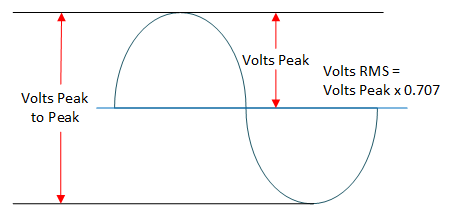
\includegraphics[scale=1]{vrms} % first figure itself
	\caption{Measurement of Vrms}
	\label{blck}
\end{figure}

Conversion for a sine wave with a zero volt offset (like that in mains or line power) is performed as follows:

\begin{enumerate}
	\item Find the peak to peak voltage  ( Volts Peak to Peak )
	\item Divide the peak to peak voltage by two to get peak voltage (Volts Peak)
	\item Multiply the peak voltage by 0.707 to yield rms volts (Volts RMS)
\end{enumerate}

Having Calculated RMS voltage,  is simply a matter of multiplying by the scale factor of the particular current sensor to yield the RMS value of the current being measured which can then be multiplied by the AC Voltage value in order to give the value of the Total Power Drawn.

\begin{equation}
I_r_m_s = \frac{V_p_p \times 0.707 \times Scale Factor}{2} 
\end{equation}

\begin{equation}
P = I_r_m_s \times 230
\end{equation}

}



\section{Disaggregation Algorithms}
Most NLIM systems provide implementations of two common benchmark
disaggregation algorithms: Steady State Analysis and Combinatorial Optimisation(CO).

\subsection{Steady State Analysis}
The NILM methods based on steady-state analysis make use of steady-state features that are derived
under the steady-state operation of the appliances. Real power (P) and Reactive power (Q) are two of the
most commonly used steady state signatures in NILM  for tracking On/Off operation of appliances.
The real power is the amount of energy consumed by an appliance during its operation. If the load is
purely resistive then the current and voltage waveforms will always be in phase and there will be no
reactive energy. For a purely reactive load the phase shift will be 90 degrees, and there will be no transfer of real
power. On the other hand, due to inductive and capacitive elements of the load, there is always a phase
shift between current and voltage waveforms that generates or consumes a reactive power respectively.

\begin{figure}[H]
	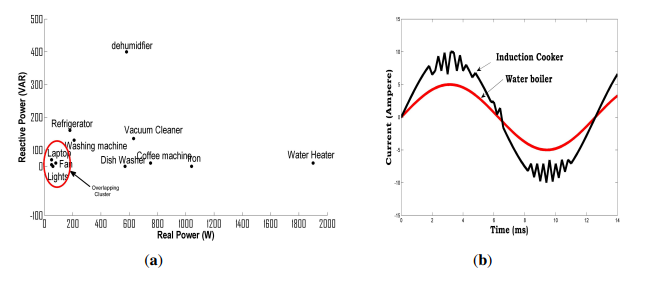
\includegraphics[scale=1]{steadystate} % first figure itself
	\caption{Load Distribution in PQ Plane and Current draw of Linear vs Non Linear Loads}
	\label{blck}
\end{figure}

Researchers have tried to disaggregate load using real power as a single feature and found
out that high-power appliances with distinctive power draw characteristics such as electrical heaters and
water pumps can be easily identified from the aggregated measurements. However this method does
not take into account appliances with similar power draw characteristics. In addition, simultaneous state
transitions of appliances leads to erroneous results. In order to address some of these issues, high power appliances can easily be differentiated
by analyzing the step changes in real and reactive power features.

\subsection{Combinational Optimization(CO)}

Combinational Optimization finds the optimal combination of appliance states, which minimizes the difference between the sum of the predicted appliance power and the observed aggregate power, subject to a set of appliance models. Since each time slice is considered as a separate optimisation problem, each time slice is assumed to be independent.
The complexity of disaggregation for T time slices is: 

\begin{equation}
N_C_o_m_b_i_n_a_t_i_o_n_s = K ^ N
\end{equation}

where N is the number of appliances and
K is the number of appliance states.

Since the complexity of CO is exponential in the number of appliances, the approach is only computationally tractable for a small number of modelled appliances. The error can be minimized by choosing the combination whose calculated power draw is the closest to the measured power drawn.


\section{Public Datasets}

Apart from a common evaluation metric there is also a lack of reference dataset on which the
performance of algorithm can be compared. It is quite obvious that the output of the load disaggregation
algorithm is dependent on the source data, which often varies either due to difference in the number
and type of appliances used in the experiment or due to the hardware used to extract the load signatures. In order to draw meaningful performance comparison of various NILM techniques,
the availability of common datasets is critical. Motivated by this, recently the Reference Energy Disaggregation Data Set (REDD) and the Building-Level fUlly labeled Electricity Disaggregation dataset (BLUED) have been made publicly available in order to facilitate the researchers in the development and evaluation of new load disaggregation algorithms. The datasets contain high-frequency and low-frequency household power measurements primarily for the evaluation of steady-state as well as transient state NILM methods.

\subsection{Reference Energy Disaggregation Dataset (REDD)}
The data contains power consumption from real
homes, for the whole house as well as for each individual circuit in
the house (labeled by the main type of appliance on that circuit).
The data is intended for use in developing disaggregation methods, which
can predict, from only the whole-home signal, which devices are being
used. The REDD data set contains two main types of home electricity data:
high-frequency current/voltage waveform data of the two power mains
(as well as the voltage signal for a single phase), and
lower-frequency power data including the mains and individual,
labeled circuits in the house. 

\subsection{Building-Level fUlly labeled Electricity Disaggregation (BLUED) Dataset}
The BLUED dataset consists of voltage and current measurements for a single family residence in the United States, sampled at 12 kHz for a whole week. Every state transition of each appliance in the home during this time was labeled and time-stamped, providing the necessary ground truth for the evaluation of event-based algorithms. 















 
 
 
 
 
 
 
 
 
 
 

 
 
 
 
 
 
 


%\input{modifications.tex}
\chapter{Hardware:}
\section{Raspberry Pi 3}{
	\begin{figure}[H]
		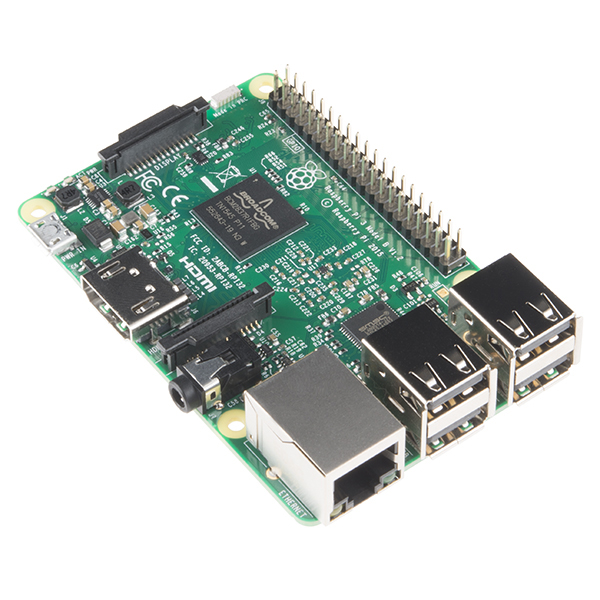
\includegraphics[scale=2]{images/rpi.jpg}
		\centering
		% first figure itself
		\caption{Raspberry Pi 3}
		\label{trans}
	\end{figure}
	The Raspberry Pi 3 is the third generation Raspberry Pi. This powerful
    credit-card sized single board computer can be used for many applications
    and supersedes the Raspberry Pi 2 Model. Whilst maintaining the popular board format the Raspberry Pi 3 Model
    B brings you a more powerful processer, 10x faster than the first generation
    Raspberry Pi. Additionally it adds wireless LAN & Bluetooth connectivity
    making it the ideal solution for powerful connected designs. It has a HDMI (rev 1.3 & 1.4 Composite RCA (PAL and NTSC).It uses Broadcom BCM2387 chipset with a
    1.2GHz Quad-Core ARM Cortex-A53 and 802.11 b/g/n Wireless LAN and Bluetooth 4.1 (Bluetooth Classic and LE). It also has a 1GB LPDDR2 memory. Operating System Boots from Micro SD card, running a version of the Linux operating system or
    Windows 10 IoT.
	%\begin{equation}
	%	C = 0.7 \times I /(\Delta V \times F)
	%\end{equation}
	
}
\section{ACS712 Module Current Sensor}{
	\begin{figure}[H]
	    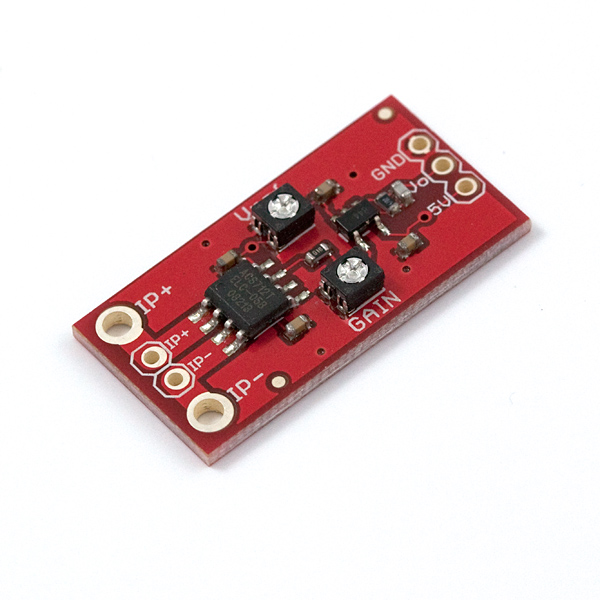
\includegraphics[scale=0.5]{images/acs712.jpg}
	    \centering
	    \caption{ACS712}
	    \label{ACS712}
	\end{figure}
	
	\begin{figure}[H]
	    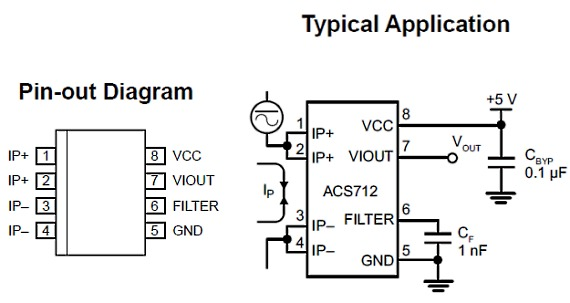
\includegraphics[scale=0.75]{PinDiagrams.jpg}
	    \centering
	    \caption{ACS712 Block Diagram}
	    \label{fig:my_label}
	\end{figure}
	The Allegro ACS712 provides economical and precise solutions for AC or DC current sensing in industrial, commercial, and communications systems.The device consists of a precise, low-offset, linear Hall circuit with a copper conduction path located near the surface of the die. Applied current flowing through this copper conduction path generates a magnetic field which the Hall IC converts into a proportional voltage. Device accuracy is optimized through the close proximity of the magnetic signal to the Hall transducer. A precise, proportional voltage is provided by the low-offset, chopper-stabilized BiCMOS Hall IC, which is programmed for accuracy after packaging. The internal resistance of this conductive path is 1.2 mΩ typical, providing low power loss. The thickness of the copper conductor allows survival of the device at up to 5× overcurrent conditions. The terminals of the conductive path are electrically isolated from the signal leads (pins 5 through 8). This allows the ACS712 to be used in applications requiring electrical isolation without the use of opto-isolators or other costly isolation techniques. It requires a 4.5-5.5V power supply. It takes input current of 0-30A and produces output voltage of 2.5-5V.
}

\section{ADC ADS1115}{
\begin{figure}[H]
		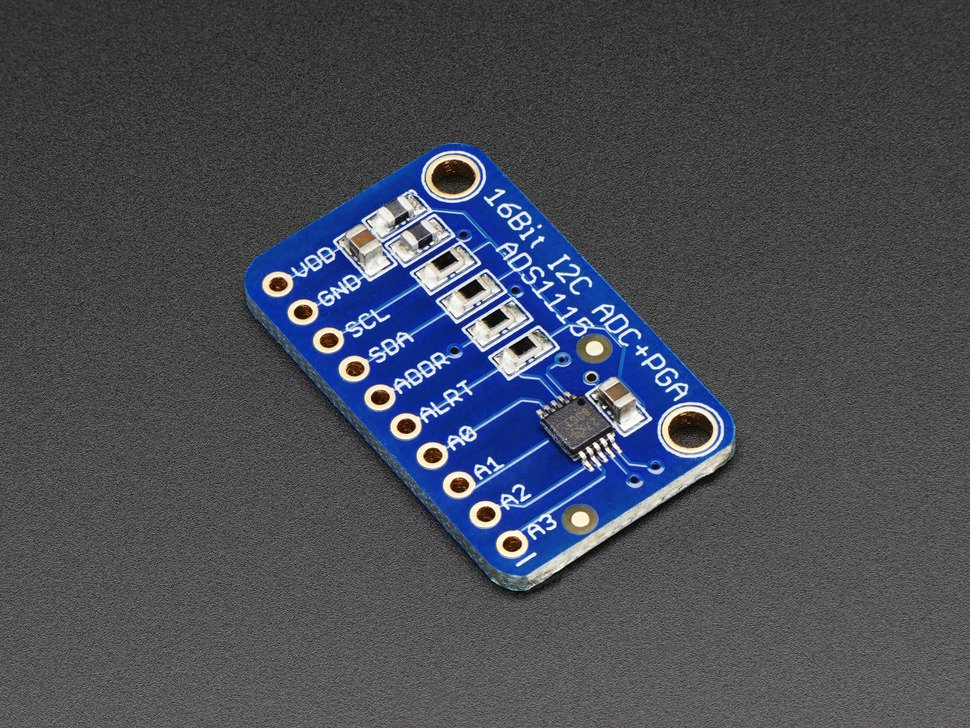
\includegraphics[scale=0.5]{images/ads1115.jpg}
		\centering
		% first figure itself
		\caption{Raspberry Pi 3}
		\label{trans}
	\end{figure}

For microcontrollers without an analog-to-digital converter or when you want a higher-precision ADC, the ADS1115 provides 16-bit precision at 860 samples/second over I2C. The chip can be configured as 4 single-ended input channels, or two differential channels. As a nice bonus, it even includes a programmable gain amplifier, up to x16, to help boost up smaller single/differential signals to the full range. We like this ADC because it can run from 2V to 5V power/logic, can measure a large range of signals and its super easy to use. It is a great general purpose 16 bit converter.

The chip's fairly small so it comes on a breakout board with ferrites to keep the AVDD and AGND quiet. Interfacing is done via I2C. The address can be changed to one of four options so you can have up to 4 ADS1115's connected on a single 2-wire I2C bus for 16 single ended inputs.

}
\section{Current Transformer}{

\begin{figure}[H]
	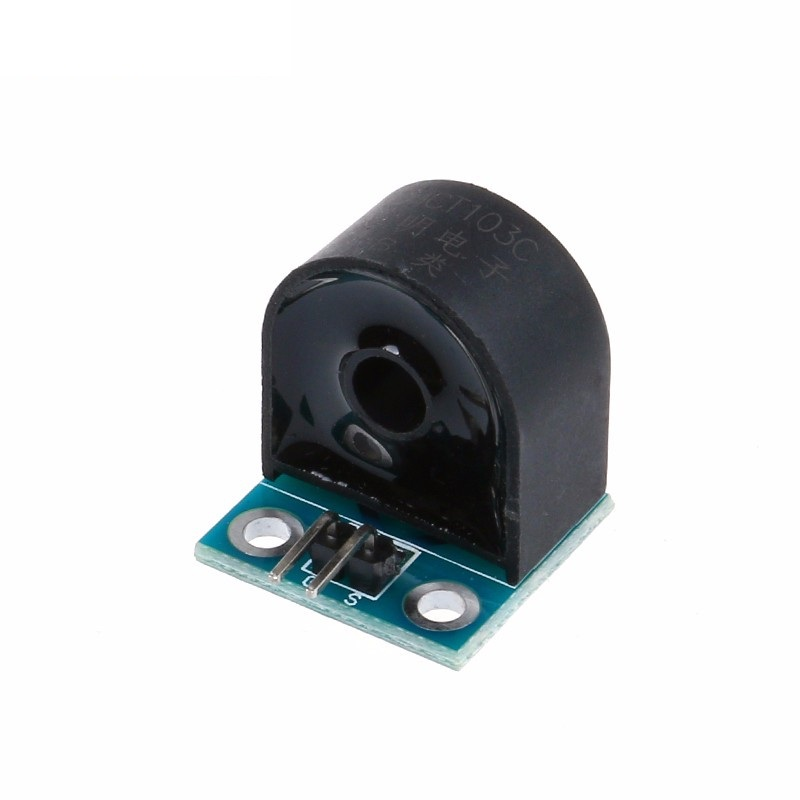
\includegraphics[scale=0.45]{images/CT2.jpg}
	\centering
	
	% first figure itself
	\caption{Current Transformer}
	\label{Current Transformer}
\end{figure}
Current transformers can perform circuit control, measure current for power measurement and control, and perform roles for safety protection and current limiting. They can also cause circuit events to occur when the monitored current reaches a specified level. Current monitoring is necessary at frequencies from the 50 Hz/60 Hz power line to the higher frequencies of switchmode transformers that range into the hundreds of kilohertz.

The object with current transformers is to think in terms of current transformation rather than voltage ratios. Current ratios are the inverse of voltage ratios. The thing to remember about transformers is that Pout = (Pin — transformer power losses). With this in mind, let's assume we had an ideal loss-less transformer in which Pout = Pin. Since power is voltage times current, this product must be the same on the output as it is on the input. This implies that a 1:10 step-up transformer with the voltage stepped up by a factor of 10 results in an output current reduced by a factor of 10. This is what happens on a current transformer. If a transformer had a one-turn primary and a ten-turn secondary, each amp in the primary results in 0.1A in the secondary, or a 10:1 current ratio. It's exactly the inverse of the voltage ratio — preserving volt times current product.

How can we use this transformer and knowledge to produce something useful? Normally, an engineer wants to produce an output on the secondary proportional to the primary current. Quite often, this output is in volts output per amp of primary current. The device that monitors this output voltage can be calibrated to produce the desired results when the voltage reaches a specified level.

A burden resistor connected across the secondary produces an output voltage proportional to the resistor value, based on the amount of current flowing through it. With our 1:10 turns ratio transformer that produces a 10:1 current ratio, a burden resistor can be selected to produce the voltage we want. If 1A on the primary produces 0.1A on the secondary, then by Ohm's law, 0.1 times the burden resistor will result in an output voltage per amp.

Many voltage transformers have adjusted ratios that produce the desired output voltage and compensate for losses. The turns-ratios or actual turns aren't the primary concern of the end-user. Only the voltage output and possibly regulation and other loss parameters may be of concern. With current transformers, the user must know the current ratio to use the transformer. The knowledge of amps in per amps out is the basis for use of the current transformer. Quite often, the end users provide the primary with a wire through the center of the transformer. They must know what secondary turns are to determine what their output current will be. Generally, in catalogues, the turns of the transformers are provided as a specification for use.

With this knowledge, the user can choose the burden resistor to produce their desired output voltage. The output current of 0.1A for a 1A primary on the 1:10 turns ratio transformer will produce 0.1 V/A across a 1Ω burden resistor, 1V per amp across a 10Ω burden and 10V per amp across a 100Ω burden resistor.

The Smart Energy Monitor uses a Current Transformer with a 1:1000 turns ratio & a burden resistor of 40 Ohm.
}

\section{Voltage Transformer}{

\begin{figure}[H]
	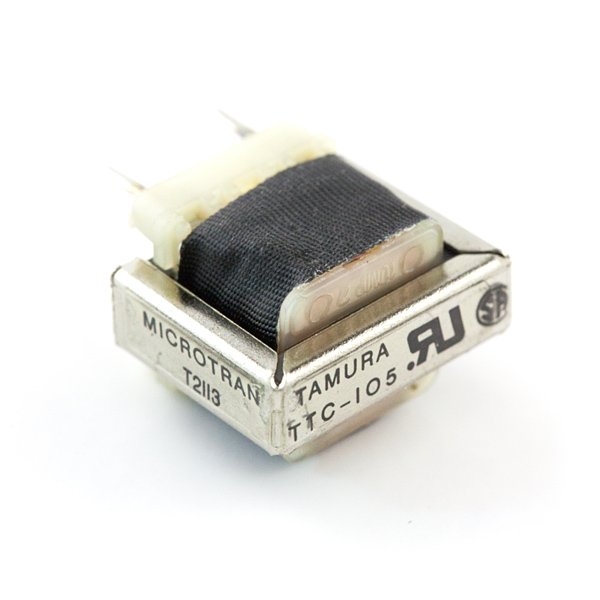
\includegraphics[width=0.9\textwidth]{images/vt.jpg} % first figure itself
	\caption{Voltage Transformer}
	\label{Voltage Transformer}
\end{figure}
Voltage transformers (VT), also called potential transformers (PT), are a parallel connected type of instrument transformer. They are designed to present negligible load to the supply being measured and have an accurate voltage ratio and phase relationship to enable accurate secondary connected metering.
The Smart Energy Monitor uses a 230:5 turns ratio voltage transformer 
}


\section{Arduino}{
\begin{figure}[H]
	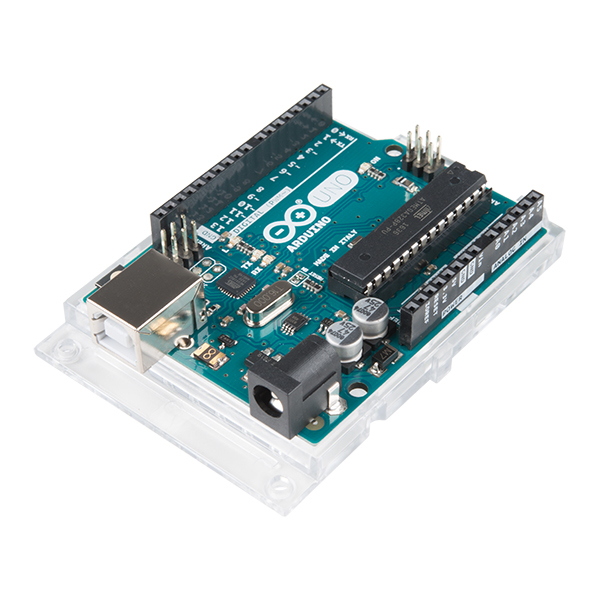
\includegraphics[width=0.9\textwidth]{images/arduino.jpg} % first figure itself
	\caption{Arduino Uno}
	\label{Arduino Uno}
\end{figure}
Arduino Uno is a microcontroller board based on the ATmega328P (datasheet). It has 14 digital input/output pins (of which 6 can be used as PWM outputs), 6 analog inputs, a 16 MHz quartz crystal, a USB connection, a power jack, an ICSP header and a reset button. 
}

\section{Comparator LM339}
{The LM339 devices consist of four independent voltage comparators that are designed to operate from a single power supply over supplies also is possible, as long as the difference between the two supplies is 2 V to 36 V, and VCC isat least 1.5 V more positive than the input common-mode voltage. Current drain is independent of the supply voltage. The outputs can be connected to the other open-collector outputs to achieve wired-AND relationships} 


\section{Operational Amplifier LM324}
{The LM324-N series consists of four independent,
high-gain, internally frequency compensated
operational amplifiers designed to operate from a
single power supply over a wide range of voltages.
Operation from split-power supplies is also possible
and the low-power supply current drain is
independent of the magnitude of the power supply
voltage.}

\section{ExOR Gate 74HC86}
{
The 74HC86 is a quad 2-input EXCLUSIVE-OR gate. Inputs include clamp diodes. This enables the use of current limiting resistors to interface inputs to voltages in excess of VCC. 
}

\chapter{Design and Implementation:}

\section{Current Difference}
{
Inorder to measure the AC Current using the current transformer we must:

\begin{enumerate}
  \item Connect only the Live wire between the AC source and the load appliances through the current transformer.
  \item Measure the peak voltage dropped across the 40 ohm burden resistor that is on the transformer output
  \item Convert that voltage across the resistor to a current by applying ohms law (I = V/R).
  \item Multiply the peak voltage by 0.707 to get and RMS Voltage across the resistor.  (0.707 as a factor only applies to Sine Waves).
  \item Multiply the RMS current by 1000 to get yield the value going through the wire being measured.  (The current transformer has a 1000 to 1 ratio).
  
\end{enumerate}

\begin{figure}[H]
	    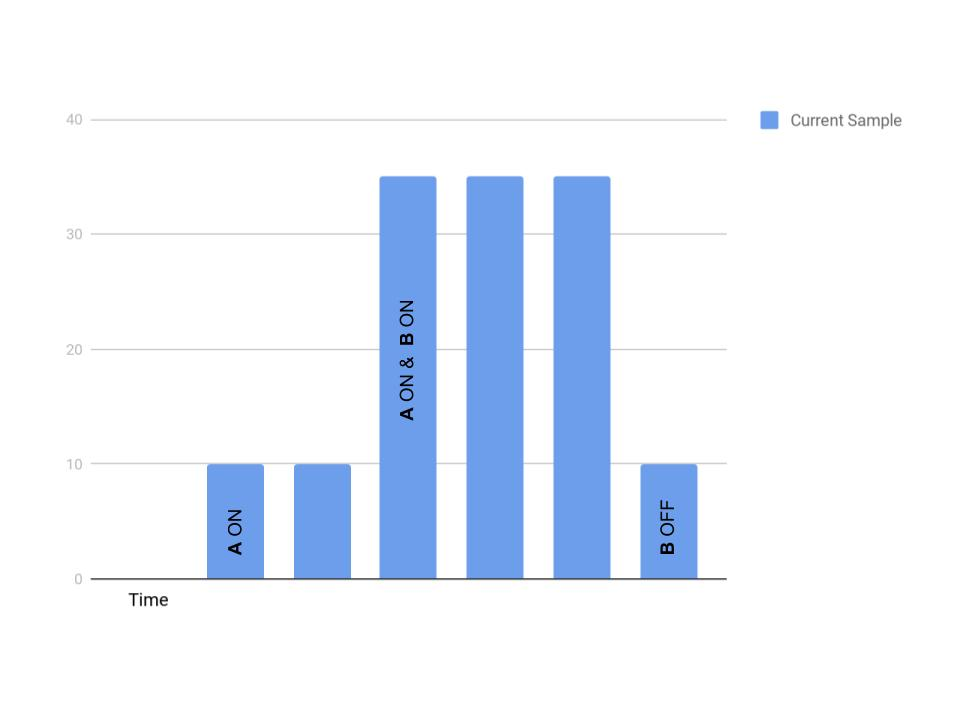
\includegraphics[scale=0.50]{images/cdiff.jpg}
	    \centering
	    \caption{Change in Current between Conscutive Samples}
	    \label{cdiff}
	\end{figure}
	

The Current drawn by the load is the first parameter used to classify the various load appliances. The current transformer is used as a current sensor which will provide us with the instantaneous value of the total current drawn by all loads connected to the Smart Energy Monitor. 
In order to get the value of the current drawn by each individual load appliance we must calculate the difference between each of the consecutive current sample. 

As shown in the above figure, we can see that when load appliance A is turned ON, the change in current is 10, when B is turned ON after A, the change in current is 25 but the total current is 35 and finally when B is turned OFF the change in current is 25 while the total current drawn is 10.

\subsection{Averaging Consecutive Current Samples}
The total change in current that occurs when a load appliance is switched ON/OFF may not be correctly reflected between the two consecutive samples. Instead the total change in current may be reflected over more than two consecutive current samples depending on the switching speed or transient time of the load appliances. Hence, occasionally large errors are produced when measuring the current difference between any two consecutive current samples.

In order to reduce the error, the sampling rate may be adjusted accordingly. But calibrating the sampling rate may be difficult as various load appliances have different transient times as well as the time taken for different software instructions may differ with different hardware and sensors.

\centering
T_{otal} C_{urrent} =  \sum_{0}^{N}C_{urrent} S_{amples}

\begin{figure}[H]
	    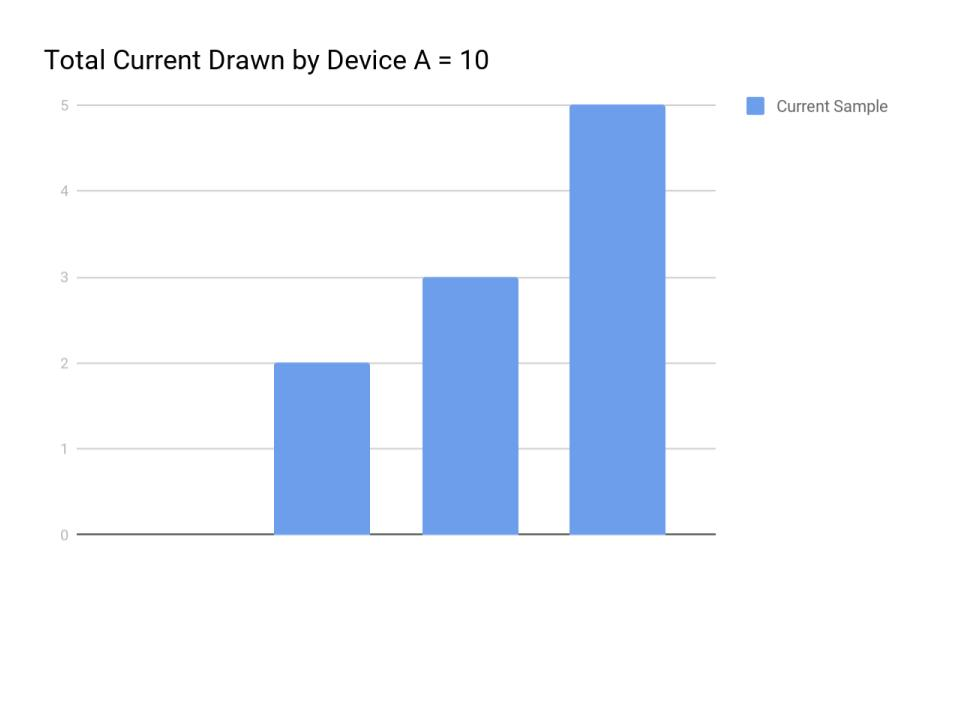
\includegraphics[scale=0.50]{images/cdiff2.jpg}
	    \centering
	    \caption{Sum of N Current Samples}
	    \label{cdiff}
	\end{figure}


A more efficient method for reducing this error will be to find the sum of N consecutive current samples such that the sum of all the error is zero(or close to zero). The user may have to wait for a very short duration before the next load appliance can be switched ON/OFF. The small error that remains will not come into effect as the classification algorithm will rule it out based on the mean and standard deviation values of all the labelled data.

As shown in the above figure, load appliance A during its transient state as a total current change of 10. But this value is not reflected between any two consecutive current samples. Instead the change in current observed between any two consecutive current samples for load appliance A is 2,3 and 5 respectively. Hence the value of error produced will be either 3 or 5. But if we take the sum of N consecutive samples where in N in this case is equal to 3, then we will get an error value of 0.
}

\section{Active Power and Reactive Power}
{
Using only the current drawn by a load as a classification parameter has the following limitation:
\begin{itemize}
  \item If two or more completely different load appliances(different applications) draw the same amount of current, the current difference between N consecutive samples for both the devices may be equal which may produce an incorrect result.
 \end{itemize}
 
 \begin{figure}[H]
	    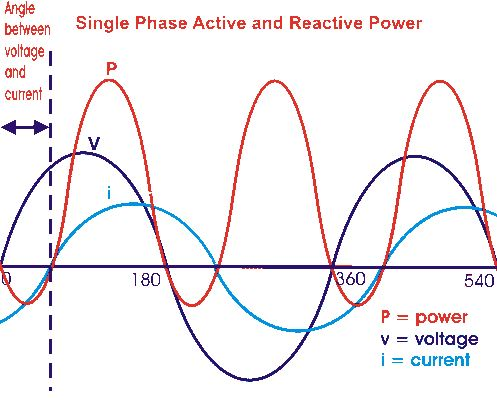
\includegraphics[scale=1]{images/phasediff.JPG}
	    \centering
	    \caption{Phase Difference between Voltage and Current}
	    \label{cdiff}
	\end{figure}

 
 Hence in order to more accurately differentiate between load appliances which draw the same amount of current, we also consider the value of active power and reactive power drawn by each individual load appliance. It will be highly unlikely that two completely different load appliances with different applications and uses have the same current drawn as well as Active Power and Reactive Power values.
}

\section{Phase Angle}
{

\begin{figure}[H]
	    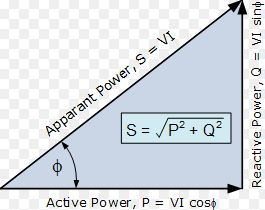
\includegraphics[scale=1]{images/triangle.jpg}
	    \centering
	    \caption{Power Triangle}
	    \label{cdiff}
	\end{figure}

\begin{equation}
    Active\ Power = P = V_{RMS}I_{RMS}\cos\phi
\end{equation}


\begin{equation}
    Reactive\ Power = Q = V_{RMS}I_{RMS}\sin\phi
\end{equation}

\begin{equation}
    Apparent\ Power = S = \sqrt{P^{2}+Q^{2}}
\end{equation}

In order to calculate the Active Power and Reactive Power drawn by load appliances, we must first find the phase difference between the voltage and current.
We do this by implementing a zero cross detector for both the voltage and current. 


\begin{figure}[H]
	    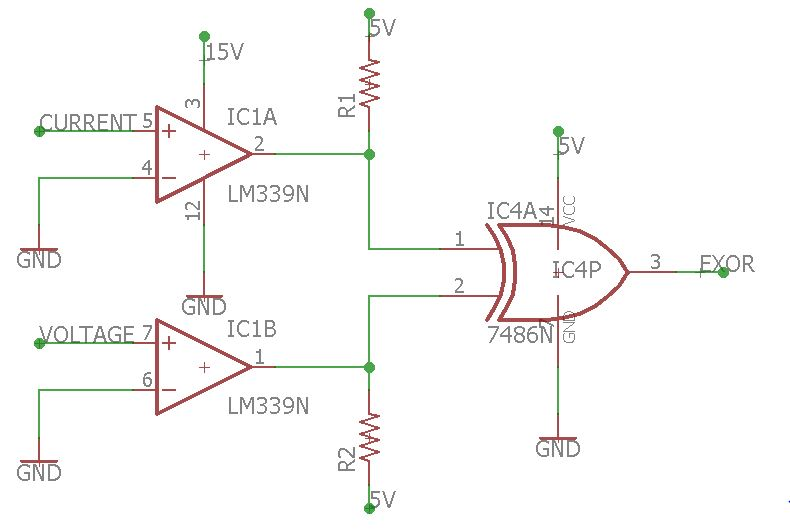
\includegraphics[scale=0.75]{images/zcd.jpg}
	    \centering
	    \caption{Zero Cross Detector}
	    \label{zcd}
	\end{figure}


The zero cross detector is built using the LM339. 

\begin{equation}
    Y = (Voltage + Current) \cdot (\overline{Voltage}+\overline{Current})
\end{equation}

The output of the zero cross detectors is fed to the Ex-OR gate of the 7486 EXOR IC which will produce pulses when there is a phase shift. i.e. The two logic levels of the inputs to the EXOR gate are not equal to each other. 

\begin{equation}
    Phase\ Angle = \phi=360\times Frequency\times \triangle Time
\end{equation}

The time period(t) of these pulses can be be used to find the phase angle between the voltage and current waveforms.

\subsection{Current Amplification}
The current transformer has a turns ratio of 1:1000. Hence if the current drawn by the load is around 1A, the output of the current transformer will be 1mA. Many load appliances draw currents far lower than 1A and hence the resulting voltage developed across the burden resistor connected to the current transformer may be lower than the input common mode voltage of the comparator. 


\begin{figure}[H]
	    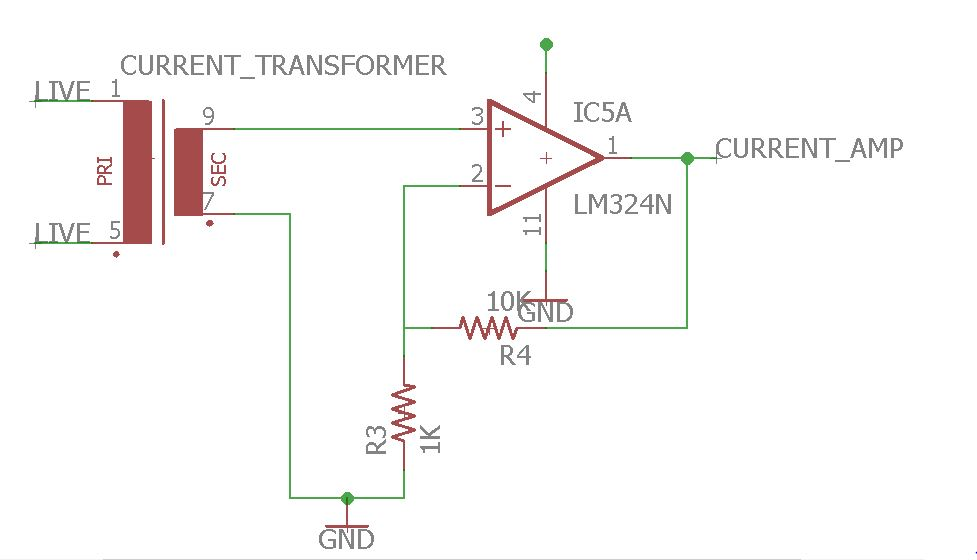
\includegraphics[scale=0.70]{images/iamp.jpg}
	    \centering
	    \caption{Current Signal Amplifier}
	    \label{iamp}
	\end{figure}


In order to produce a voltage that is greater than the input common mode voltage of the comparator, output voltage across the burden resistor must be amplified. A non inverting amplifier must be used so that there is no effect on the values of phase angle between voltage and current.

\begin{equation}
Gain = 1+ \frac{R_{f}}{R_{1}} 
\end{equation}

The LM324 has an operational amplifier which can be configured as an Non Inverting amplifier with suitable gain for the purpose of amplifying the current signal. 
}
\section{Serial Communication}
{
The Arduino is used as a low cost ADC which can transmit data to the Raspberry Pi.
The Arduino transmits this data using Serial Communication through a USB cable. This is useful since no logic level conversion is required when compared to the I2C or GPIO communication protocols.
Data such as the current drawn as well as Active Power and Reactive Power are sent to the Raspberry Pi.
The Arduino is directly powered through its USB port. Hence no additional external power supply is required for the Arduino.


}

\section{Naive Bayes Classification}
{
The Naive Bayes algorithm is an intuitive method that uses the probabilities of each attribute belonging to each class to make a prediction. It is the supervised learning approach you would come up with if you wanted to model a predictive modeling problem probabilistically.

Naive bayes simplifies the calculation of probabilities by assuming that the probability of each attribute belonging to a given class value is independent of all other attributes. This is a strong assumption but results in a fast and effective method.

The probability of a class value given a value of an attribute is called the conditional probability. By multiplying the conditional probabilities together for each attribute for a given class value, we have a probability of a data instance belonging to that class.

To make a prediction we can calculate probabilities of the instance belonging to each class and select the class value with the highest probability.

Naive bases is often described using categorical data because it is easy to describe and calculate using ratios. A more useful version of the algorithm for our purposes supports numeric attributes and assumes the values of each numerical attribute are normally distributed (fall somewhere on a bell curve). Again, this is a strong assumption, but still gives robust results.
}

\subsection{Creating the Dataset}{
The dataset is created by measuring the values of the current drawn, active power and reacive power drawn by individual load appliances. These data points are then used to identify the device.
The change in these parameters must follow the following condition to be considered as valid data point:
\begin{itemize}
    \item The increase in any classification parameter(current drawn, active power and reactive power drawn) when a load appliance is turned ON must be equal to decrease in that classification parameter when the load appliance is turned OFF.
    \item The values of the data points of a particular load appliance must remain the same even if other devices are active. This must apply for all combinations of load appliances and their individual states.
\end{itemize}

The valid data points have to be labelled according to the load appliance state. 
The data is stored in a standard CSV format table.
The more validated & labelled data within the dataset will make the predicted result more accurate. 

}

\subsection{Impelementation of Classification Algorithm}{
The implementation of most classification algorithms involve the following processes:

\begin{enumerate}
  \item \textbf{Handle Data:} Load the data from CSV file and split it into training and test datasets. Split the data into a training dataset that Naive Bayes can use to make predictions and a test dataset that we can use to evaluate the accuracy of the model. 
  
  \begin{equation}
      Training\ Data = 0.67 \times Dataset\ Size
  \end{equation}
  
   \begin{equation}
      Testing\ Data = 0.33 \times Dataset\ Size
  \end{equation}
 
  
  
  We need to split the data set randomly into train and datasets with a ratio of 67 percent train and 33 percent test (this is a common ratio for testing an algorithm on a dataset).


 \item \textbf{Summarize Data: } Summarize the properties in the training dataset so that we can calculate probabilities and make predictions.
 \item \textbf{Make a Prediction:} Use the summaries of the dataset to generate a single prediction.
 \item \textbf{Make Test Data Predictions:} Generate predictions given a test dataset and a summarized training dataset.
\item \textbf{Evaluate Accuracy:} Evaluate the accuracy of predictions made for a test dataset as the percentage correct out of all predictions made.
\item \textbf{Tie it Together:} Use all of the code elements to present a complete and standalone implementation of the Naive Bayes algorithm.
 
\end{enumerate}
}


\subsection{Data Summarizing}{
The naive bayes model is comprised of a summary of the data in the training dataset. This summary is then used when making predictions.

The summary of the training data collected involves the mean and the standard deviation for each attribute, by class value.

These are required when making predictions to calculate the probability of specific attribute values belonging to each class value.

We can break the preparation of this summary data down into the following sub-tasks:

\begin{enumerate}
    \item \textbf{Separate Data By Class:} The first task is to separate the training dataset instances by class value so that we can calculate statistics for each class. We can do that by creating a map of each class value to a list of instances that belong to that class and sort the entire dataset of instances into the appropriate lists.
\item \textbf{Calculate Mean:} We need to calculate the mean of each attribute for a class value.

\begin{equation}
Mean\ of\ each\ Attribute\ for\ Class\ Value = \frac{Sum\ of\ all\ Attributes}{Total\ Number\ of\ Attributes}
\end{equation}

The mean is the central middle or central tendency of the data, and we will use it as the middle of our gaussian distribution when calculating probabilities.

We also need to calculate the standard deviation of each attribute for a class value. The standard deviation describes the variation of spread of the data, and we will use it to characterize the expected spread of each attribute in our Gaussian distribution when calculating probabilities.

\begin{equation}
    Standard\ Deviation\ of\ each\ Attribute\ for\ Class\ Value = \sigma = \sqrt{\frac{\sum_0^n (x-\overline{Mean})^{2}}{n}}
\end{equation}

In the above equation n = The number of attributes.
The standard deviation is calculated as the square root of the variance. The variance is calculated as the average of the squared differences for each attribute value from the mean. 

\item \textbf{Summarize Dataset:} Now we have the tools to summarize a dataset. For a given list of instances (for a class value) we can calculate the mean and the standard deviation for each attribute.

\item \textbf{Summarize Dataset:} Now we have the tools to summarize a dataset. For a given list of instances (for a class value) we can calculate the mean and the standard deviation for each attribute.

\item \textbf{Summarize Attributes By Class:} We can pull it all together by first separating our training dataset into instances grouped by class. Then calculate the summaries for each attribute. 


\end{enumerate}

}

\subsection{Making Predictions}
We are now ready to make predictions using the summaries prepared from our training data. Making predictions involves calculating the probability that a given data instance belongs to each class, then selecting the class with the largest probability as the prediction.

We can divide this part into the following tasks:

\begin{enumerate}
    \item \textbf{Calculate Gaussian Probability Density Function:} We can use a Gaussian function to estimate the probability of a given attribute value, given the known mean and standard deviation for the attribute estimated from the training data.


\begin{equation}
    Gaussian\ Probability = \frac{1}{\sqrt{2\pi \sigma^{2}}} \times Exponent
\end{equation}

\begin{equation}
    Exponent = e^{-\frac{(x-Mean)^{2}}{2 \sigma^{2}}}
\end{equation}



Given that the attribute summaries where prepared for each attribute and class value, the result is the conditional probability of a given attribute value given a class value. 

\item \textbf{Calculate Class Probabilities:} Now that we can calculate the probability of an attribute belonging to a class, we can combine the probabilities of all of the attribute values for a data instance and come up with a probability of the entire data instance belonging to the class.

We combine probabilities together by multiplying them. 

\item \textbf{Making a Prediction:}
Now that can calculate the probability of a data instance belonging to each class value, we can look for the largest probability and return the associated class.
Finally, we can estimate the accuracy of the model by making predictions for each data instance in our test dataset. This will return a list of predictions for each test instance.


\item \textbf{Estimating Accuracy:} 

\begin{equation}
Accuracy = \frac{Number\ of\ Accurate\ Predictions}{Size\ of\ the\ Testing\ Dataset}\times100
\end{equation}

The predictions can be compared to the class values in the test dataset and a classification accuracy can be calculated as an accuracy ratio between 0& and 100%.

\end{enumerate}



\section{Additional Classification Parameters}
The more number of parameters used in classification algorithms will further improve the quality of the dataset.

These additional parameters are non numerical values. Hence a decision tree algorithm along with a Naive Bayes classification must be implemented when considering any non numerical parameters.

\begin{figure}[H]
	    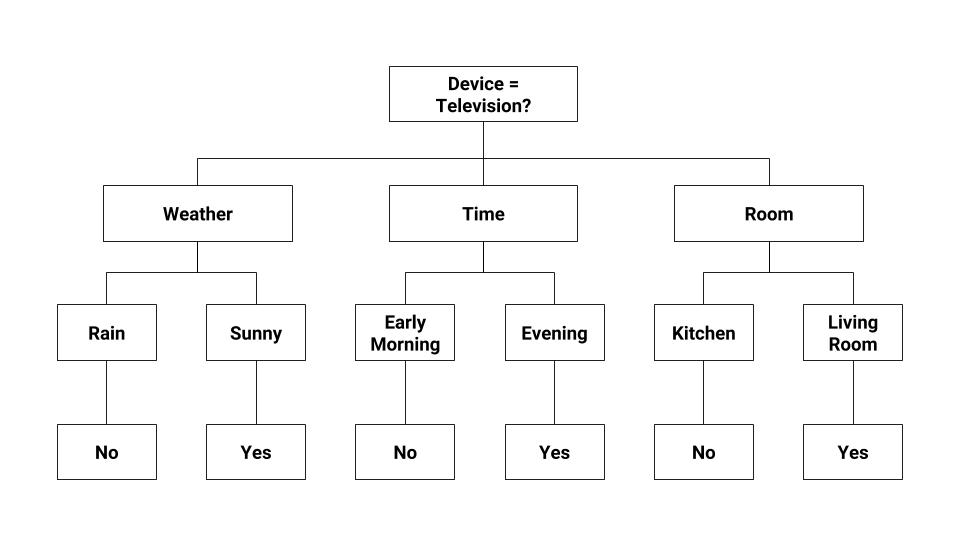
\includegraphics[scale=0.45]{images/tree.jpg}
	    \centering
	    \caption{Electricity Tariff}
	    \label{cost}
	\end{figure}


Hence in addition to the current, active power and reactive power classification parameters, we propose the use of additional parameters such as:

\subsection{Weather}
The current weather may determine the state of the device. For example, when the temperature is low and the residents begin to feel cold during the winter, the likelihood of the Air Conditioner being on is highly unlikely.
The weather data will have to be calibrated according to a particular geographic location

\subsection{Time & Day}
The time of the day can also be used to determine the state of the device. For example, during the day and during the night(sleep time 1 A.M. to 6 A.M.), the likelihood of the use of high power lighting is highly unlikely.

In some cases the day of the week can be used as an additional classification parameter. For example, during weekends, more people are present at home(weekdays spent at Work,college,etc), hence the likelihood of the use of entertainment systems such as Television and Gaming systems during the midday as well as the likelihood of the use of kitchen appliances during the midday will significantly increase. 

This may vary from household to household but with a large dataset of mixed households, this parameter may become very useful.

The time & day data will have to be calibrated according to a particular timezone.

\subsection{Room Location}
{
Certain load appliances have fixed places within an household. By creating another parameter which takes into account the location of a load appliance within the household can also improve the quality of the dataset. 
For example, most households have refrigerators & microwaves in the kitchen, water heating geysers in the bathroom, televisions & home theatre systems in the living room. On the other hand, the likelihood of an Air Conditioner within a bathroom will be highly unlikely. 

This will indeed require additional hardware and separate current sensors per room.
}

\section{Voltage Calibration}
{


\begin{figure}[H]
	    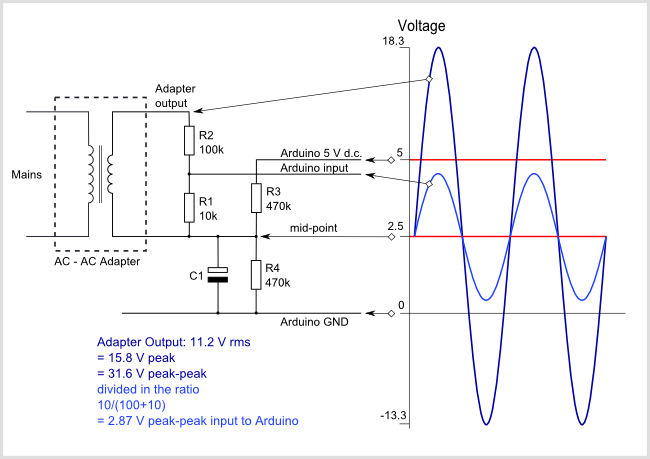
\includegraphics[scale=0.70]{images/volt.png}
	    \centering
	    \caption{Voltage Calibration}
	    \label{volt}
	\end{figure}

\begin{equation}
    Peak\ Output\ Voltage = \frac{R_1} {R_1 + R_2} \times Peak\ Input\ Voltage
\end{equation}

The standard household AC voltage provided by electricity distributors varies from 220V to 240V. 
Hence the voltage value will vary depending on the location, electricity distributor and even in some cases voltage fluctuations.
In order taken into account such voltage variations, the voltage transformer is used to calibrate the household voltage once the Smart Energy Monitor has been installed.  
}

\section{Estimating Electricity Bill}

\begin{figure}[H]
	    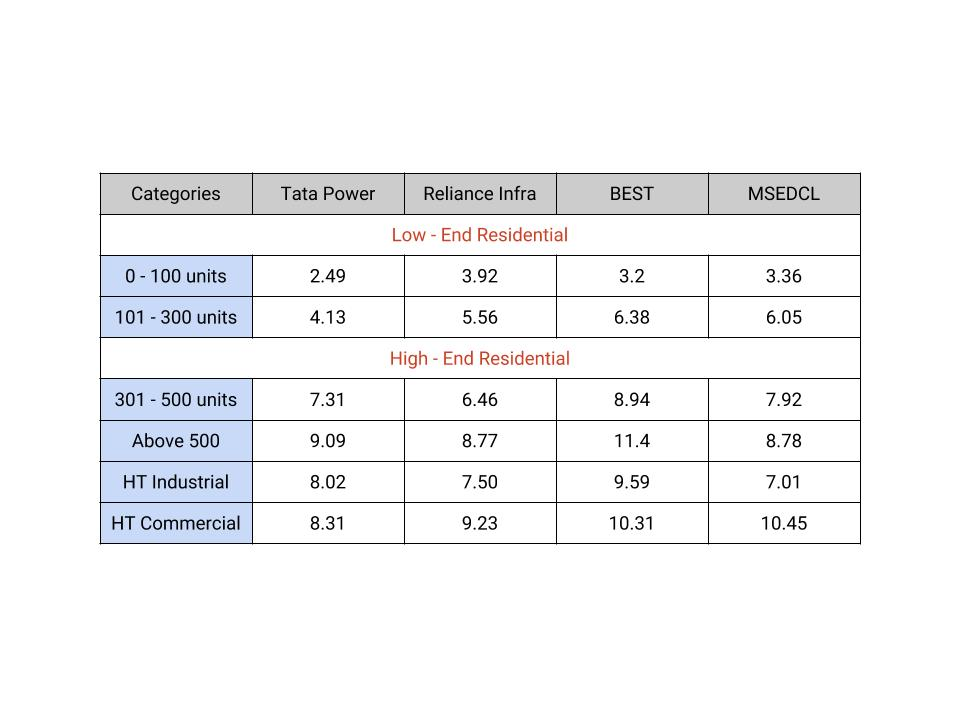
\includegraphics[scale=0.45]{images/cost.jpg}
	    \centering
	    \caption{Electricity Tariff}
	    \label{cost}
	\end{figure}

\begin{equation}
    Monthly\ Electricity\ Bill = Number\ of\ Units\ Consumed \times Cost\ per\ Unit
\end{equation}

By calculating the total number of units (1KWh = 1unit) consumed per month we can estimate the electricity bill for that month. The cost per unit of electricity will vary based on the electricity distributor as well as the number of units consumed.


\section{User Interface}
{}


\subsection{Flask Microframework}
{The user interface uses a Python Micro-Framework called Flask which is used to build web applications.

The Flask framework encodes the real time Python Variables into a JavaScript Object Notation(JSON) string.

The JSON string is then read into the HTML file using Asynchronous JavaScript And XML(AJAX) requests. 

These requests are periodically refreshed using the Auto-Refresh function in AJAX.}
\begin{figure}[H]
	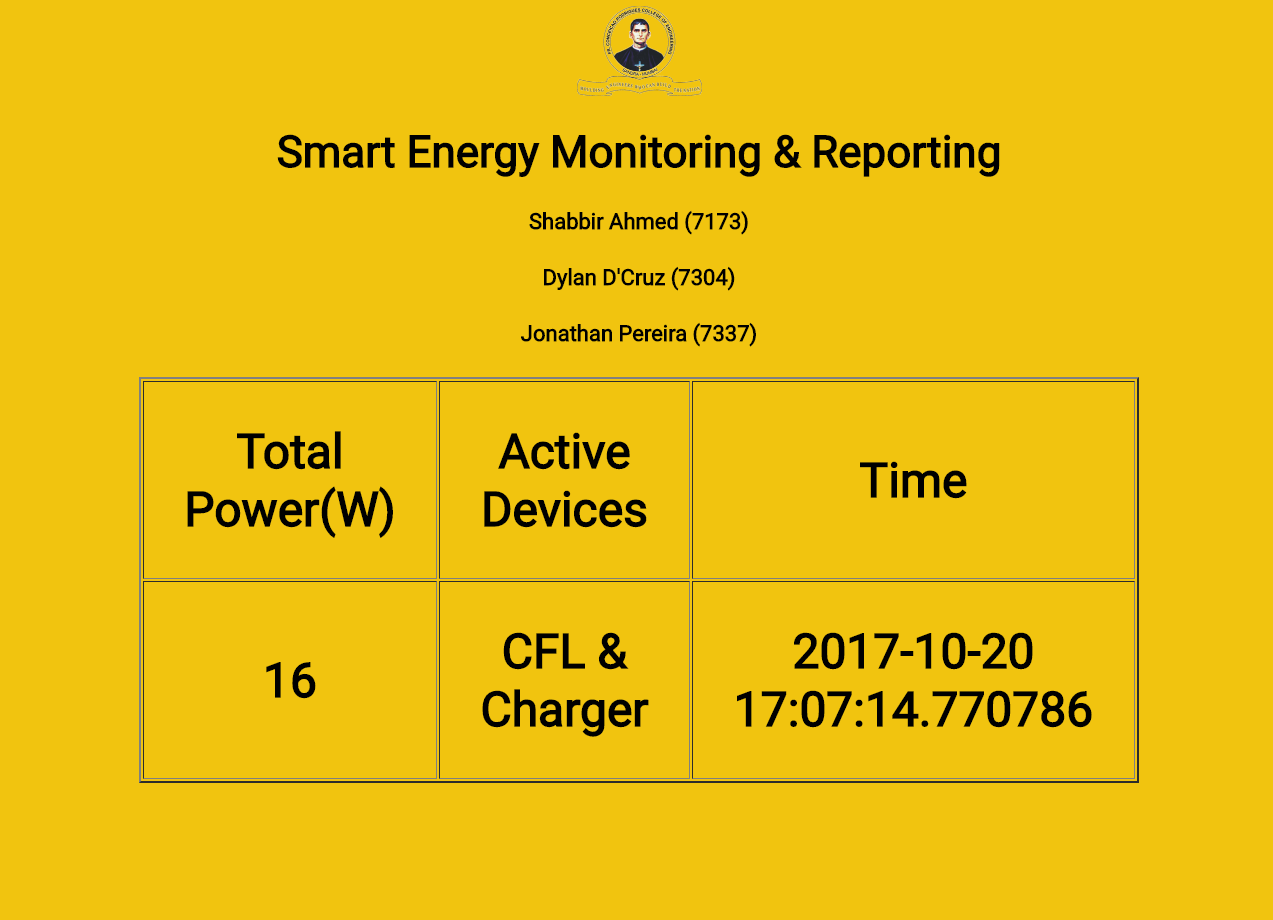
\includegraphics[width=0.9\textwidth]{Demo1.PNG} % first figure itself
	\caption{HTML-Based UI}
	\label{UI}
\end{figure}
{The user interface displays various system parameters such as Total Power being Consumed, Active Devices and the Real Time Clock. Additional parameters such as Estimated Monthly Electricity bill can be added in the future.}


\subsection{Dash Framework}{
\begin{figure}[H]
	    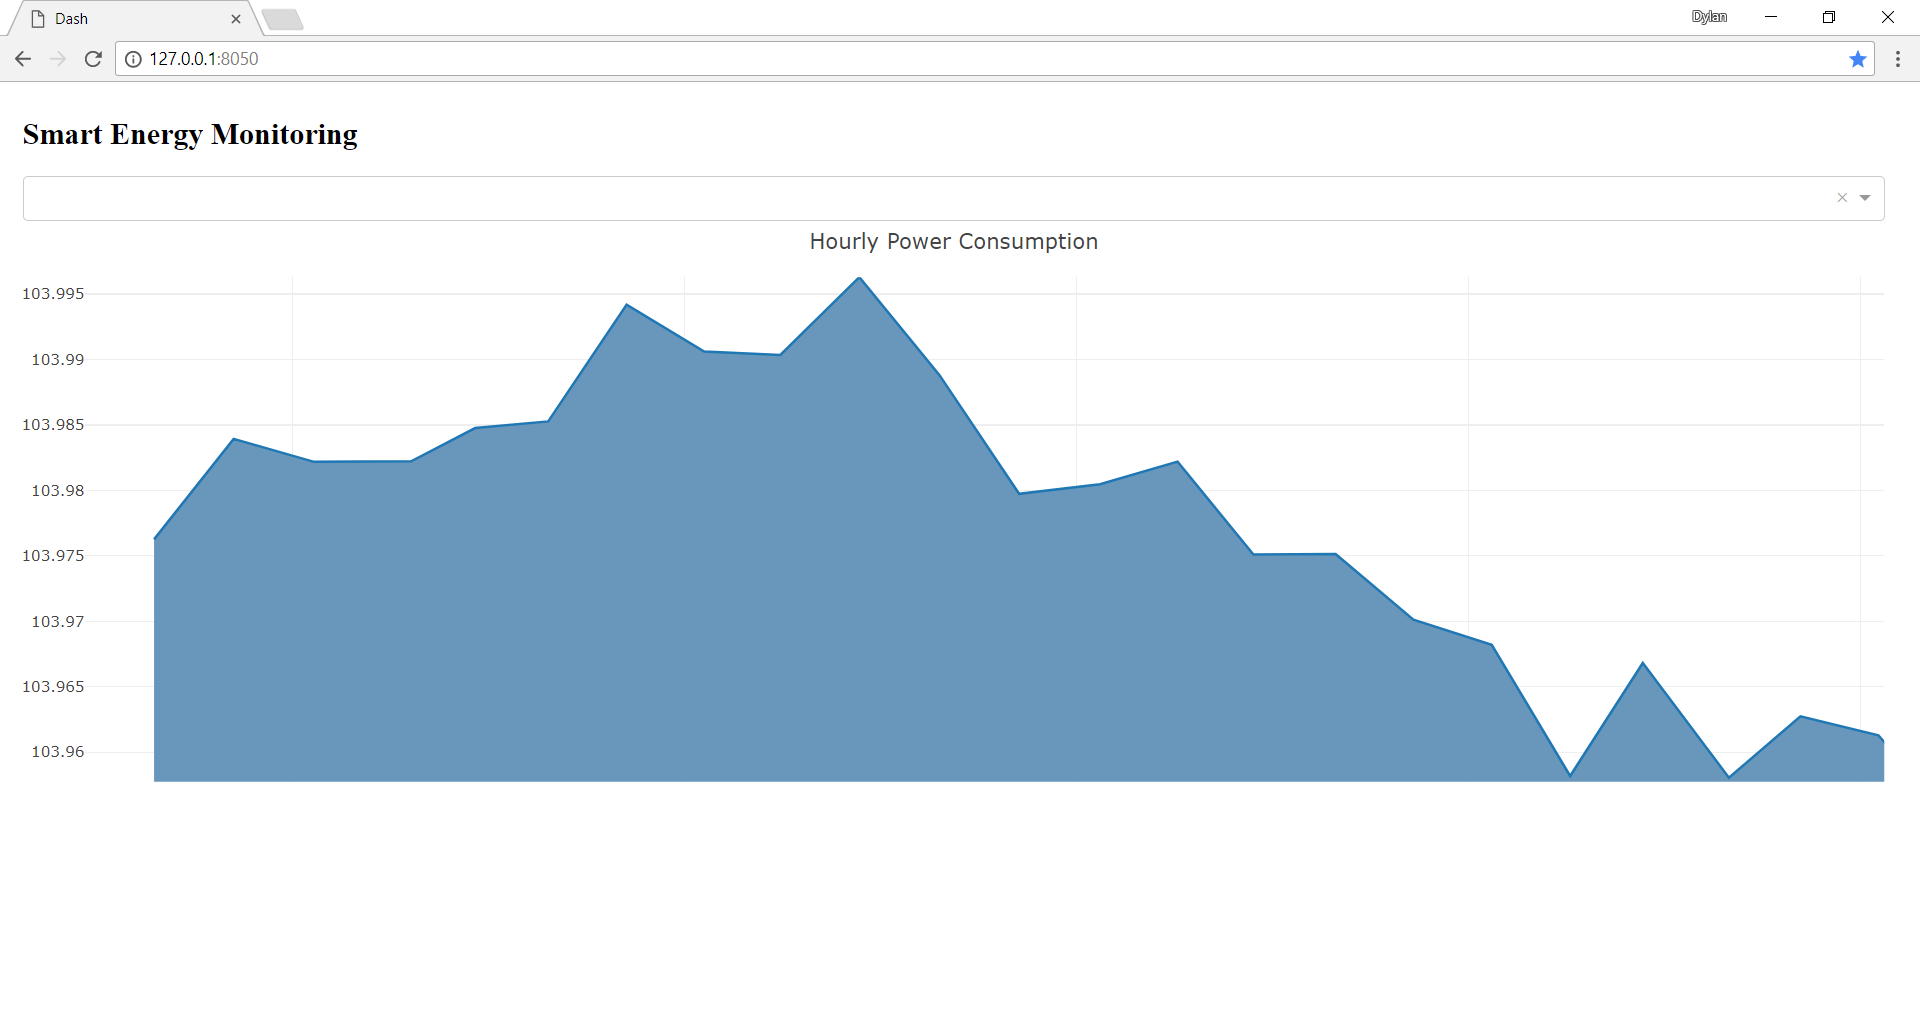
\includegraphics[scale=0.25]{images/dash.jpg}
	    \centering
	    \caption{Hourly Power Consumption over a 24hr period cycle using Dash}
	    \label{Dash}
	\end{figure}
	



Dash is a Python framework for building analytical web applications. There is no JavaScript required.
Built on top of Plotly.js, React, and Flask, Dash ties modern UI elements like dropdowns, sliders, and graphs to your analytical Python code.

We plan on using Dash to plot various live graphs as well as a pie chart of the energy usage of all load appliances.
}
\chapter{Results}
\section{Observations}
The sensor is successfully interfacing with the UI using the Raspberry Pi. It is printing the estimated power consumption using output of the current sensors. Using a simple classification algorithm, we are able to determine the device or combination of devices being used in the box. This is meant to portray a room of electronic devices.
The current is being found by sampling the AC output of the sensor and finding its RMS voltage. Upon testing it is found that the output is being found with a 5 percent margin of error.

\section{Drawback }
The classification algorithm being used is only able to identify events with significantly different power consumption. For more precise identification, an algorithm must be implemented that takes other factors such as weather or time into account.
While the margin of error in current reading isn't significant as of now, for a large number of similar devices, 2-5 Watt errors will be substantial. Moreover, only considering current and taking a constant voltage will give inaccurate readings since it doesn't take into account the voltage fluctuations.

\section{New approach}
A KNN algorithm will be able to take into account other factors when identifying events. It can take the power output as well as 2 or e more factors to further aid in identifying which event is most likely to be occurring at the moment.
To improve power reading accuracy, a voltage sensor must also be implemented. Similarly, the sampling code for the current sensor must be refined to reduce error.
Finally, more features need to be added to the UI such as power consumption per device and predictive alerts that determine when a device is being used unnecessarily. There also needs to be a portable version of the interface for accessibility purposes.
%\input{test.tex}
%\input{system.tex}
%\input{implement.tex}
%\input{summary.tex}
%\input{intro.tex}
%\input{Chapter2.tex}
%\input{Stability.tex}
%\input{StateSpace.tex}
%\input{CircuitExample.tex}
%\input{SolvedEXP.tex}
%\input{FRSS.tex}
\chapter{\Large{Conclusion}} \label{con}
The system is able to successfully disaggregate the power signals and classify the active devices. 
By calculating the active time for individual load appliances, we can track the total power consumed by that device. This information can then be used to estimate the monthly electricity bill. It can also provide the user with detailed insights as to which devices are not energy efficient & can help the user track their energy usage.

\begin{thebibliography}{9}
\bibitem{opennlim} 
Nipun Batra, Jack Kelly, Oliver Parson, Haimonti Dutta, William Knottenbelt, Alex Rogers, Amarjeet Singh and Mani Srivastava
\textit{NILMTK: An Open Source Toolkit for Non-intrusive Load
            Monitoring}. 

\bibitem{nlimsensors} 
Ahmed Zoha, Alexander Gluhak, Muhammad Ali Imran, Sutharshan Rajasegarar
\textit{Non-Intrusive Load Monitoring Approaches for Disaggregated
    Energy Sensing: A Survey}. 
\\\texttt{www.mdpi.com/1424-8220/12/12/16838/pdf}

\bibitem{henryscurrent} 
Henry's Bench
\textit{How to Measure AC Current with an Arduino and an ASC712}. 
\\\texttt{http://henrysbench.capnfatz.com/henrys-bench/arduino-current-measurements/acs712-arduino-ac-current-tutorial}

\bibitem{watty} 
Watty - 
\textit{A simple way to keep track of what goes on at home}. 
\\\texttt{https://watty.io/}
            
\end{thebibliography}
%\renewcommand\bibname{References}
%\addcontentsline{toc}{chapter}{Appendix}
%\appendix
%\input{main.tex}
%\insertcode{"scilab.sci"}{A sample Scilab code} % The first argument is the script location/filename and the second is a caption for the listing
%\nocite{*}
%\renewcommand\bibname{Bibliography}
%\bibliographystyle{IEEEtran}
%\bibliography{project-ref}
%\addcontentsline{toc}{chapter}{Bibliography}
%\setcounter{toc}{-1}


\end{document}
